To study the structure of the disk, we examined the intensity profiles in \SI and polarized intensity by extracting data points along the minor axis of the disk at each wavelength. The location of the minor axis slice for each wavelength is shown in Figure \ref{fig: slice-along-minor}, the background is polarized intensity by the slice is the exact same for \SIns. Comparing the slices in both \SI and polarized intensity allows us to compare the differences in the distribution of the total light versus the polarized light from the disk.


\add{How we add the beam as a Gaussian onto the plot}
% ------------------------------------------------
\begin{figure*}[h]
  \centering
  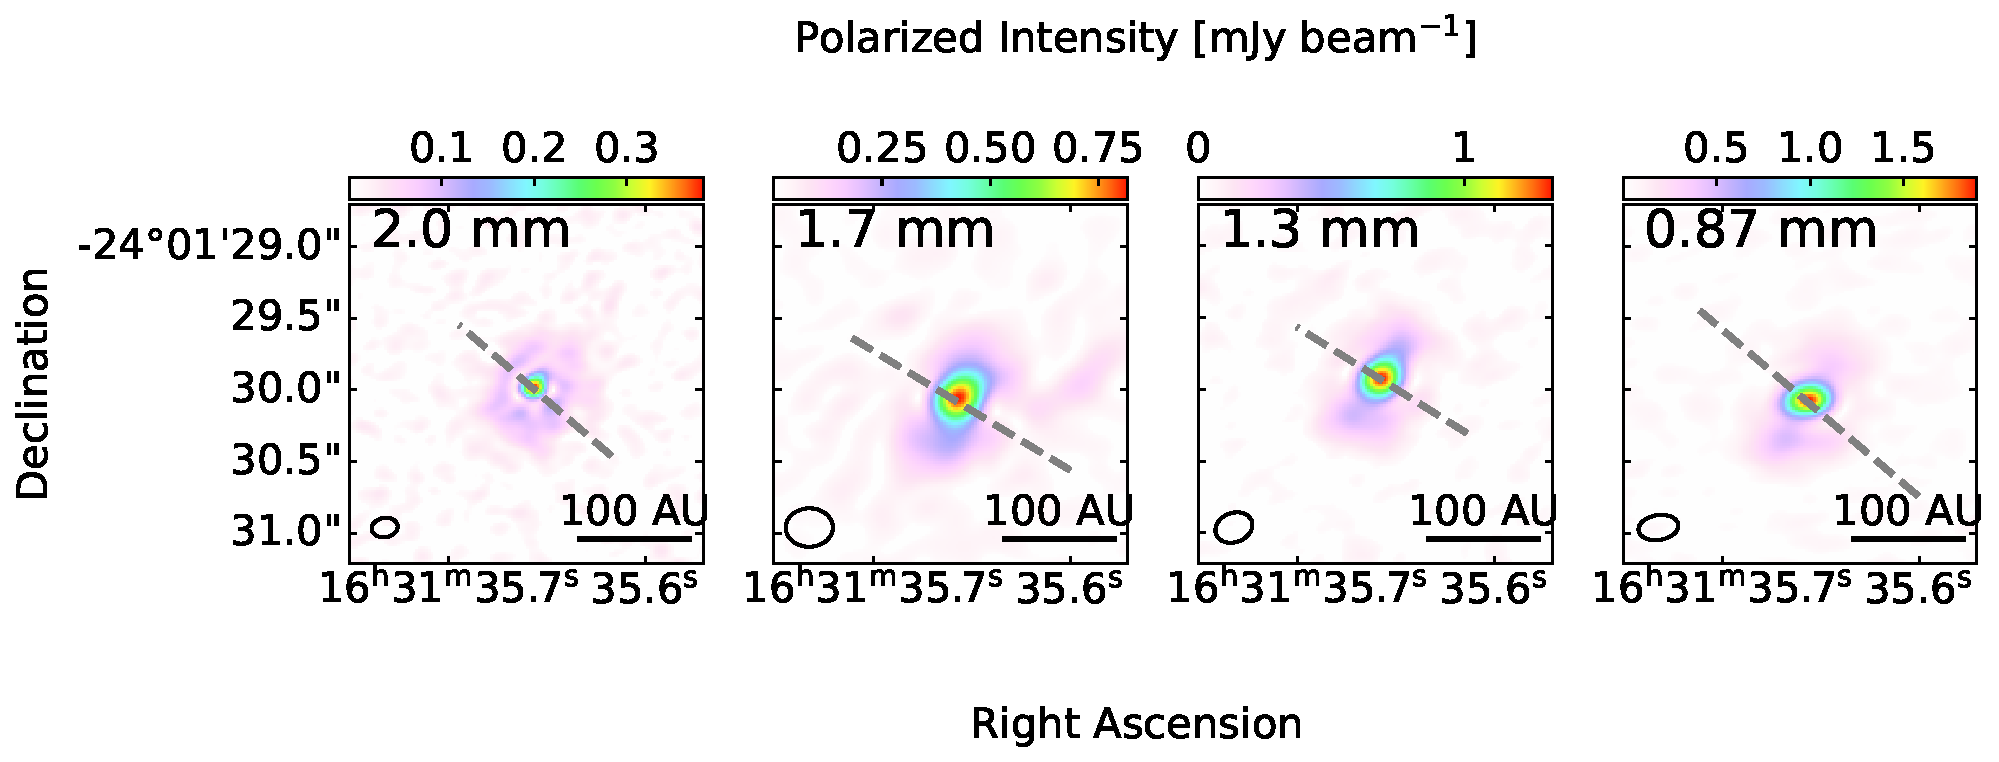
\includegraphics[width=1.1\textwidth]{WRITEUP_AND_IMAGES/IMAGES/WRITEUP/Slices/MinorAxisSliceGrid.pdf}
  \caption{\add{Caption.} Visualization of the location of the extracted minor-axis slices at each wavelength. \question{Should I take anything off of the plot? 100 AU, beam, cbar, etc.}}
  \label{fig: slice-along-minor}
\end{figure*}
% ------------------------------------------------






